\chapter{Irradiation Tests}
\label{chap:II-6-irradiation}

  The OptoHybrid will be located in a region of CMS exposed to high fluxes of particles, some of which might interact with the FPGA and generate errors in the logic. Those could in turn influence the functioning of the system and degrade its performance. To solve this issue, irradiation tests have been performed to measure the interaction cross-section of the particles with the various components of the FPGA. Two OptoHybrids have been placed in a high intensity proton beam with a dedicated firmware designed to detect errors. The two boards were each controlled by an additional OptoHybrid placed outside the test area which recorded the events and statistics. \\

  In this chapter, we provide the user with an overview of the internal architecture of an FPGA to better understand the potential sources of errors and the effects of radiation. We then describe the firmware of the irradiated and control FPGAs which has been used during the test. The setup and beam parameters of the irradiation test are reviewed before presenting the results that were obtained after analysis.

  \section{Architecture of an FPGA}

    To optimize the occupancy of the resources of the FPGA and develop code that uses the full potential of the device, a deep comprehension of the intrinsic architecture of the chip is required. Although families of FPGA differ in size and complexity, their building blocks remain the same and are described hereafter.

    \subsection{Configurable Logic Blocks}

      (CLBs) \cite{VIRTEX-CLB} are the base elements of the FPGA used to implement sequential and combinatorial logic. They are composed of two important objects: look-up tables (LUTs) and registers. LUTs are components which outputs are a function of the inputs as defined in a programmable table. They implement a truth table for every possible combination of the inputs which defines the value of the outputs. The response of a LUT to a change in the inputs is almost instantaneous. LUTs in the Xilinx Virtex-6 FPGAs can either implement functions with six inputs and a single output or functions with five inputs and two outputs. The outputs of the LUTs can, if so required by the design, be connect to registers which sample the signals at the rising edge of a given clock. Register are used for their sample-and-hold functionality which makes designs synchronous to clocks. With these two components, CLBs can implement complex functions and describe intricate systems. \\

      \begin{figure}[p!]
        \centering
        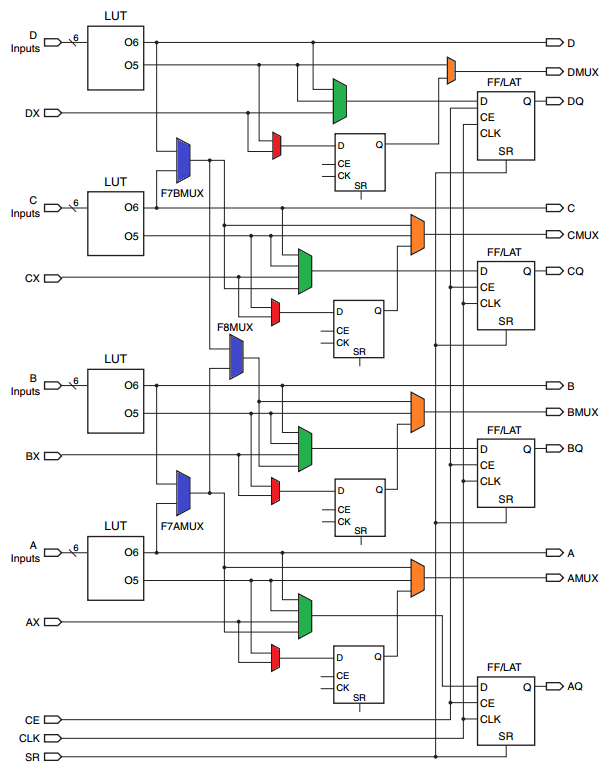
\includegraphics[width=\textwidth]{img/II-6-irradiation/clb.png}
        \caption{Simplified view of a slice composed of four LUTs on the left and eight registers on the right \cite{VIRTEX-CLB}.}
        \label{fig:II-6-clb}
      \end{figure}

      Each CLB is composed of two slices each made of four LUTs and eight register which layout is shown in Figure \ref{fig:II-6-clb}. Each LUT is connected to an input bus of six signals (A, B, C, and D inputs) and to an unbuffered output bus of a single bit (O6 to A, B, C, and D). Four additional signals enter the slice (AX, BX, CX, and DX) and are connected to multiplexers (red) which allows to buffer either the former or the second output of the LUTs (O5). The output of the same buffer is then connected to a second multiplexer (orange) which allows to select either the former or an unbuffered output of the LUTs (AMUX, BMUX, CMUX, and DMUX). Finally, a third multiplexer (green) connects a range of signals to the registers on the right which are then connected to four outputs (AQ, BQ, CQ, and DQ). Three additional multiplexers (blue) offer the possibility to mix the signals from the four LUTs to generate a wider range of logical operations. The flexibility offered by this architecture is what enables FPGAs to implement complex designs. The Xilinx Virtex-6 FPGA used in the OptoHybrid v2a (XC6VLX130T) holds 10 000 CLBs with a total of 80 000 LUTs and 160 000 registers.

    \subsection{The switching matrix}

      The inputs and outputs of the slices of the CLBs as well as of the other components of the FPGA are interconnected through the switching matrix. It is a vast network of wires and switches which are used to route signals between elements. The open or closed state of each switch is programmable and defines the routes signals follow inside the logic. Figure \ref{fig:II-6-switch} shows an element of the matrix connected to two slices (blue) along with the signals that are routed in the network (cyan). Complex designs can span a large area of the FPGA due to the high usage of logic and thus be difficult to place and route by the compiler. A technique called floorplanning is used to reduce compilation time and improve the design by constraining parts of the code to given areas in the FPGA.

      \begin{figure}[h!]
        \centering
        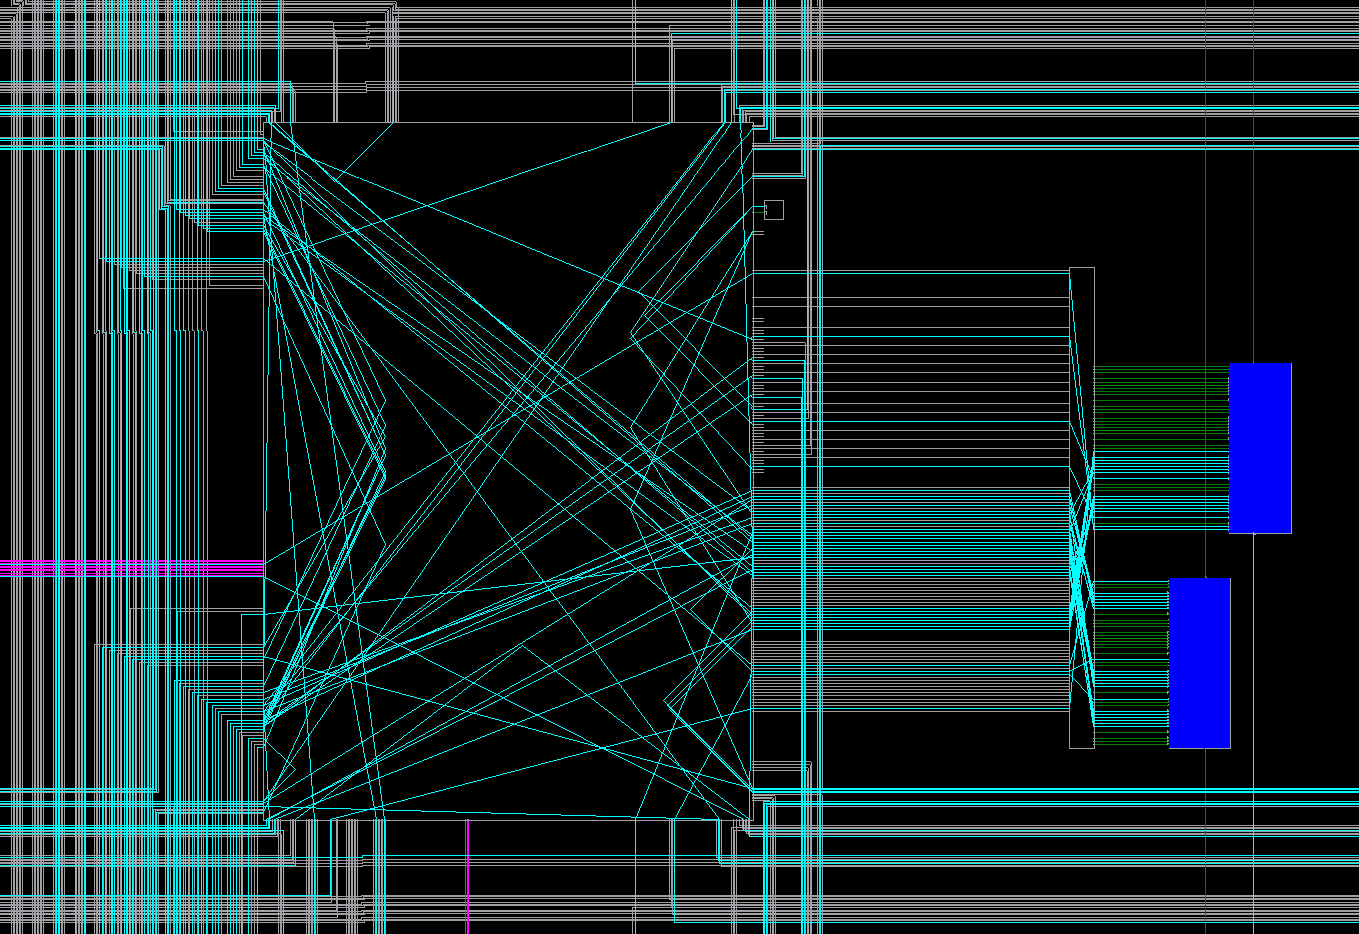
\includegraphics[width=0.8\textwidth]{img/II-6-irradiation/switch.png}
        \caption{Schematic of two slices (blue) connected to an element of the switching matrix which routes the signals (cyan) between components over the multitude of existing paths (gray).}
        \label{fig:II-6-switch}
      \end{figure}

    \subsection{Block RAM}

      Besides programmable logic, the FPGA also includes dedicated storage elements. Block RAMs \cite{VIRTEX-RAM} (BRAMs) can store up to 36 kb of data which can be configured in different ways: 32K x 1 bit, 16K x 2 bits, etc. They can also be used as First In First Out (FIFO) modules which are similar to data queues.

    \subsection{Digital Signal Processing}

      Digital Signal Processing units (DSPs) \cite{VIRTEX-DSP} are modules which perform mathematical operations using dedicated hardware elements. They are used to quickly solve problems without relying on CLBs which can consume large amount of resources to perform an equivalent task. Figure \ref{fig:II-6-dsp} shows a diagram of the DSP48E1 slices present in the Xilinx Virtex-6 family. They include a 30-bits adder, a 25-bits by 18-bits multiplier, and a programmable module which can implement either a multiplication, an addition, or a logic operation. Using the various multiplexers and configuration bits, the user can define the data paths that are followed and thus create DSP modules which meets the requirements of the design.

      \begin{figure}[h!]
        \centering
        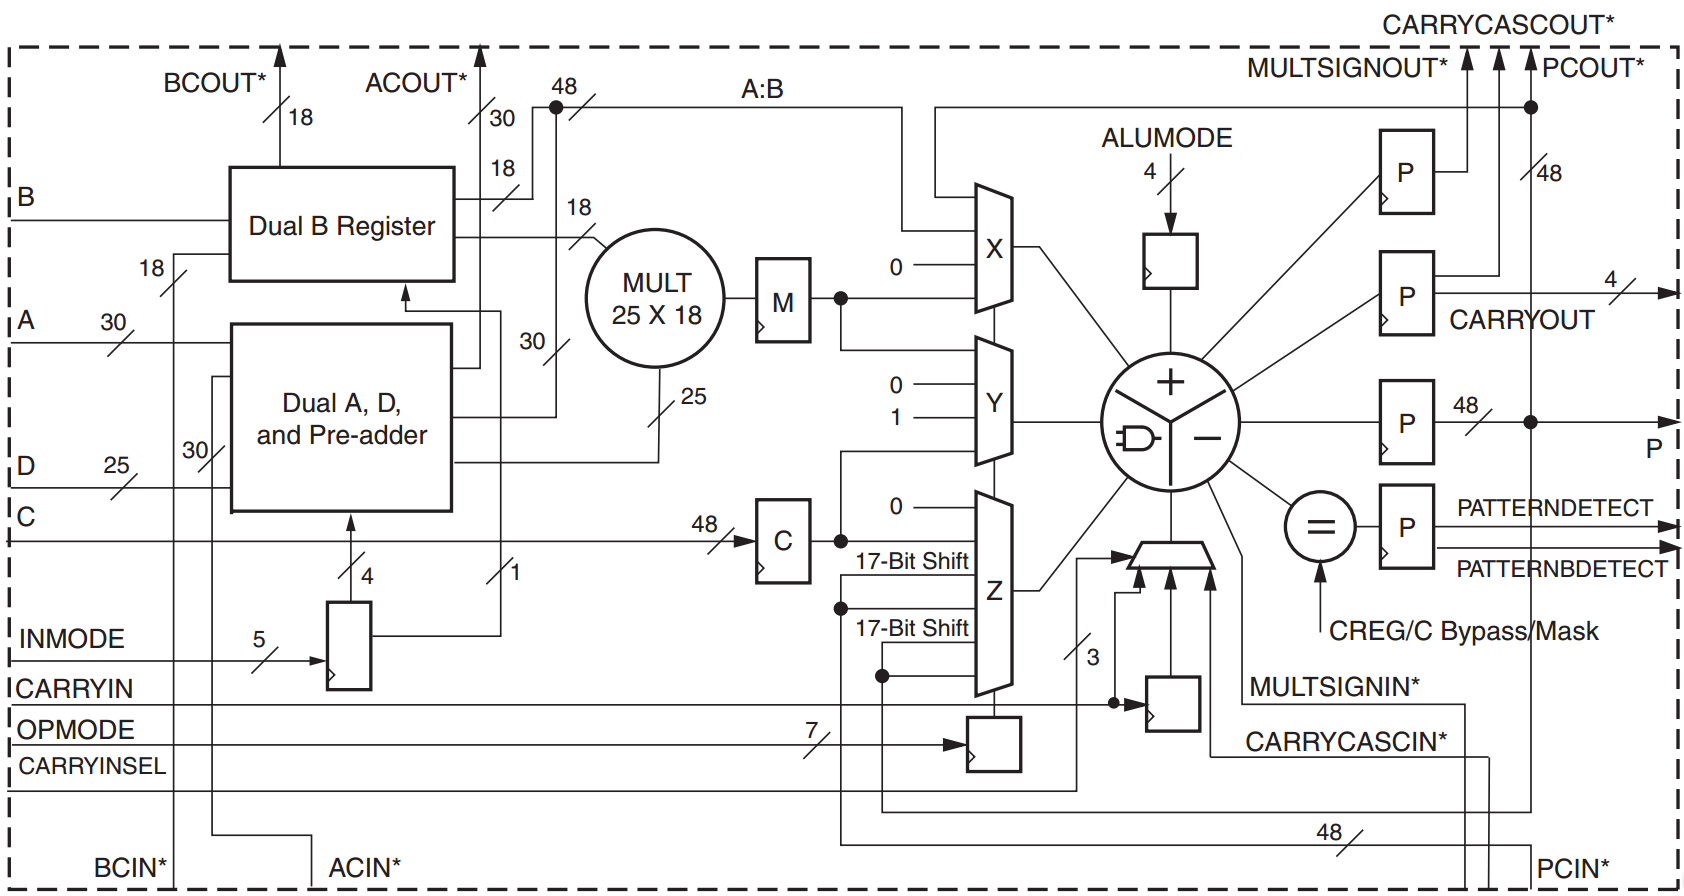
\includegraphics[width=\textwidth]{img/II-6-irradiation/dsp.png}
        \caption{Diagram of the DSP48E1 slices present in the Xilinx Virtex-6 family \cite{VIRTEX-DSP}.}
        \label{fig:II-6-dsp}
      \end{figure}

    \subsection{The configuration memory}

      The configuration memory holds the configuration of the entire FPGA and defines its behavior. It sets the truth table of the LUTs, parametrizes the DSP, creates the connection between elements, etc. It is what implements the design in the FPGA. In most FPGAs, the configuration memory is volatile and will lose its configuration upon power down or reset. To reload it, the FPGA tries to read it out of an attached memory device or remains in a blank or corrupted state if it fails to do so.

  \section{Effects of Radiation on FPGAs and Mitigation Techniques}

    When charged particles pass through an FPGA, they interact with the silicon substrate and deposit charge within the device. If the interaction takes place near a transistor, as depicted in Figure \ref{fig:II-6-transistor}, the charges can affect the functioning of the component and induce a change of state. Alternatively, particles can produce current or voltage spikes which propagate in the design. Each type of interaction results in different effects in the FPGA. The most common are the Single Event Upsets (SEU) and Single Event Transients (SET). Besides being influenced by punctual events, the FPGA will also age and degrade due to the Total Ionizing Dose (TID) of radiation.

    \begin{figure}[h!]
      \centering
      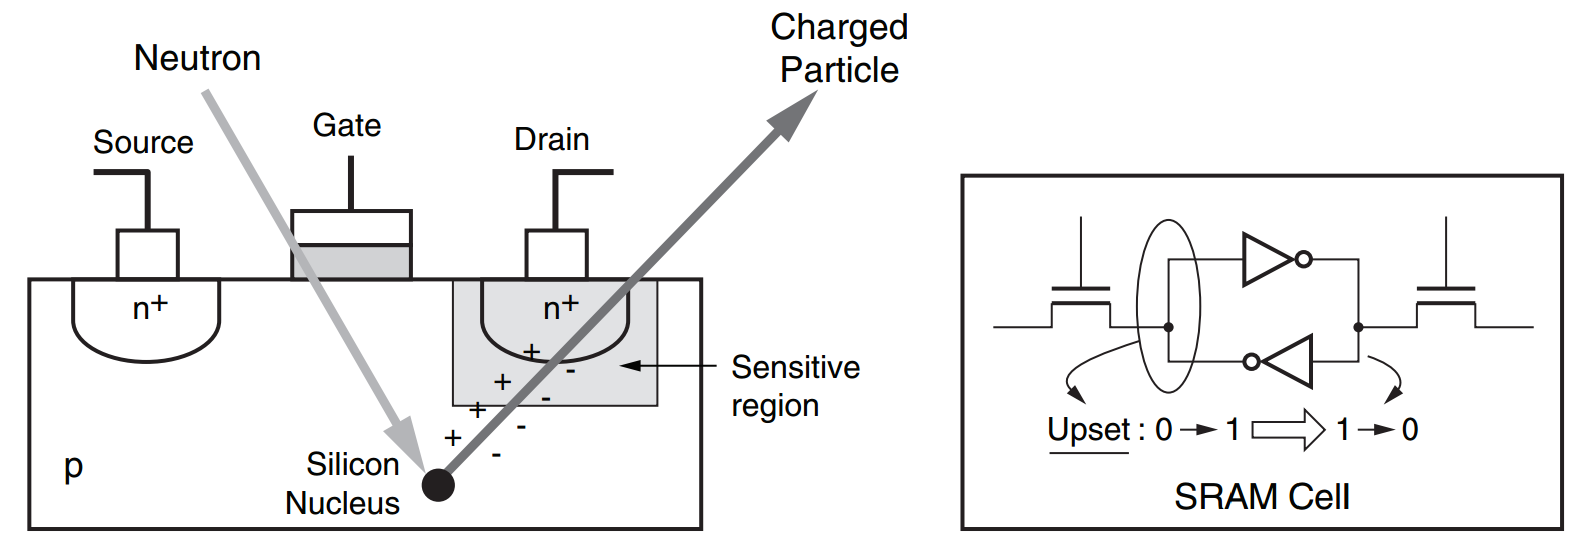
\includegraphics[width=\textwidth]{img/II-6-irradiation/transistor.png}
      \caption{Charge deposition by a charged particle inside a transistor affecting the state of the circuit \cite{XILINX-RADIATION}.}
      \label{fig:II-6-transistor}
    \end{figure}

    \subsection{Single Event Upset}

      When the charge deposited by radiation is located within a transistor, the critical voltage of the latter can be modified and a change of state occur. In case of memory cells, a change of state corresponds to a bit flip, which can influence the design. If the configuration memory is hit, the description of the CLBs, DSPs, and switch matrix will change dynamically during run time and the implemented logic will thus be affected. For BRAMs, the bit flip will occur in the data stored in memory, resulting in corrupted information. \\

      A common technique used to mitigate SEUs in CLBs and DSPs is to triplicate the logic and couple its outputs to a majority voter. First, the sequential logic is triplicated, meaning the inputs are sent to three identical modules which output is returned synchronously. The latter are then forwarded to a majority voter which performs a bit-by-bit vote and returns the most probable response. This technique can recover data if only one of the modules is affected by an SEU. In case two modules are corrupted and flip the same bit, data will be corrupted as well. Additionally, a flag can be raised by the majority voter if all three inputs are not identical, meaning an error occurred. \\

      To correct SEUs taking place in the configuration memory, the latter has to be read out by the FPGA itself. This is possible through the Soft Error Mitigation (SEM) core, a component placed inside the device which allows the firmware to analyze the data in memory and, using a two bit complement, perform a FEC on the bits. Although very effective to correct errors on the fly, this technique is time consuming due to the large amount of data to readout and can take up to several milliseconds to identify and repair and error. Furthermore, the FEC will fail to recover the data in case two bits are flipped within the same word, raising a flag that tells the system a hard reset is needed. \\

      Finally, SEUs occurring in BRAMs can be corrected using a two complements FEC which can recover single bit errors and detect double bit errors.

    \subsection{Single Event Transients}

      If the event affects combinatorial logic, a spike in current or voltage can be produced and propagate within the design. When coupled to sequential logic, such errors can be easily recovered from if their duration is small in comparison to the frequency of the clock used to run the circuit. Unless the error is produced exactly at the sampling time of the registers, it is not stored and thus mitigated.

    \subsection{Total Ionizing Dose}

      With time, the FPGA ages under the effects of radiation and malfunctions might appear. As charges get trapped in the substrate, transistors inside the device suffer from a shift in the threshold voltage of the gate and of leakage currents. This in turn affects the design, either by rendering data cells useless or by causing changes in the gate states.

  \section{Firmware Design for the Irradiated FPGA}

    The firmware of the irradiated FPGA is designed to use a maximum of the available resources and transmit any error detected during run time. Specific firmware has been developed to test the CLBs, BRAMs, DSPs, and SEM. To optimize the design, floorplanning is used to divide the FPGA in ten regions running identical code. This prevents the compiler from placing elements in different sectors of the device and thus increase routing resources. Figure \ref{fig:II-6-floorplanning} depicts how the design occupies the FPGA: the image on the left represents the FPGA sectors labeled XaYb composed of CLBs in dark blue, BRAMs in red, and DSPs in green; the image in the middle highlights the resources used by the design; and the image on the right shows how the firmware developed for each function occupies the FPGA with CLBs in blue, BRAMs in yellow, DSPs in red, SEM in purple, and the communication protocol in green.

    \begin{sidewaysfigure}[p!]
      \centering
      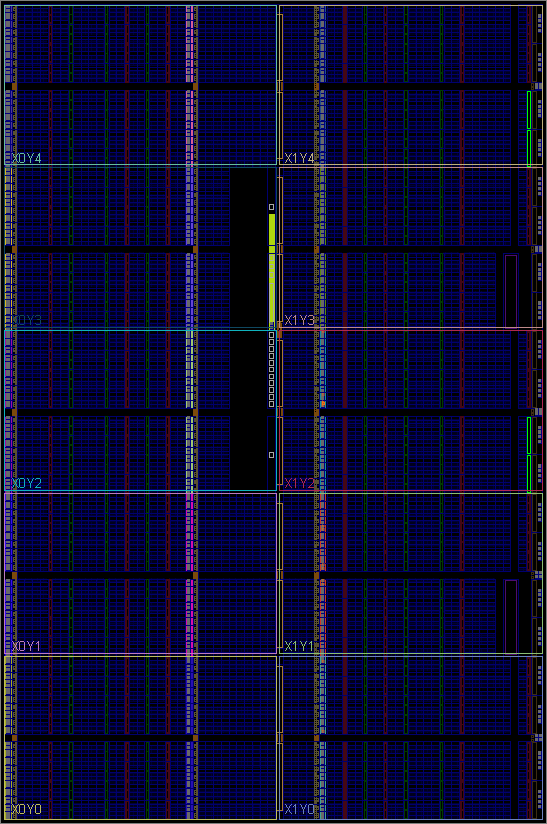
\includegraphics[width=0.32\textwidth]{img/II-6-irradiation/fpga-empty.png}
      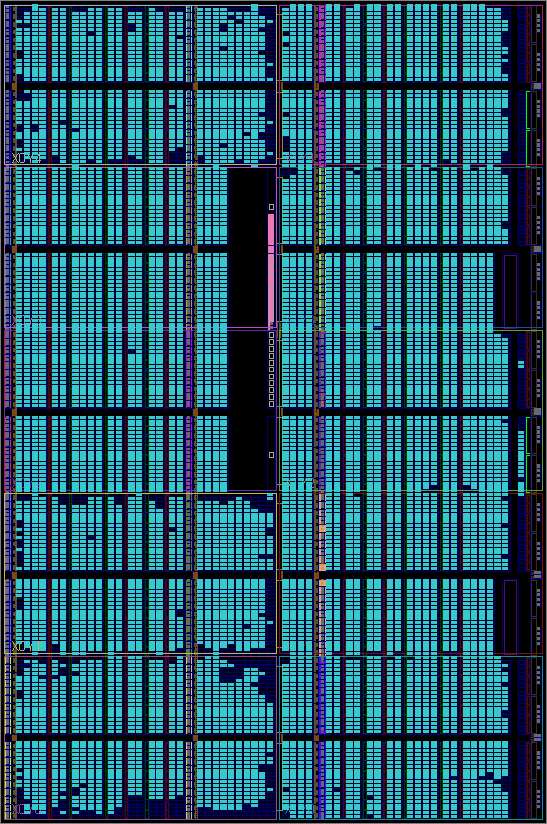
\includegraphics[width=0.32\textwidth]{img/II-6-irradiation/fpga-used.png}
      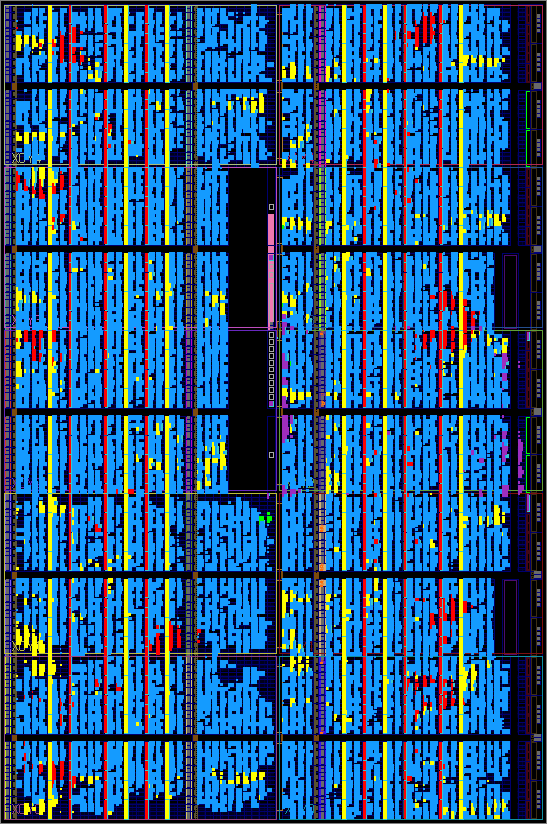
\includegraphics[width=0.32\textwidth]{img/II-6-irradiation/fpga-color.png}
      \caption{Schematic view of the occupancy of the FPGA. Left: sectors of the FPGA labeled XaYb composed of CLBs in dark blue, BRAMs in red, and DSPs in green. Middle: highlight of the resources used by the design. Right: occupancy of the code developed to test the CLBs in blue, BRAMs in yellow, DSPs in red, SEM in purple, and the communication protocol in green.}
      \label{fig:II-6-floorplanning}
    \end{sidewaysfigure}

    \subsection{Configurable Logic Block}

      To test the CLBs, an algorithm performing logic operations and bit swapping on a 32-bit word is triplicated and connected to a majority voter to form a level-1 module. Three level-1 modules are connected together to another majority voter to form a level-2 module. The level-1 modules are used to detect errors in the CLBs and the level-2 modules to signal when the triplication technique fails to recover errors. The 32-bit word fed to the algorithm is generated by shifting a word every clock cycle. The same data is provided to all modules meaning that it is not susceptible to SEUs. \\

      Each of the ten sectors of the FPGA contains 19 level-2 modules and 3 additional level-1 modules for a total occupancy of the FPGA of 80\%. Within each sector the flags of the level-1 and level-2 modules are gathered and sent to the communication module which forwards information to the control FPGA.

    \subsection{Block RAM}

      In Xilinx Virtex-6 FPGAs, some of the BRAM components are equipped with error detection and correction features. These can detect double bit flips and correct for single bit flips. 90\% of the available BRAMs, namely 240 components, are used and constantly written to and read from in order to detect SEUs happening inside the memory cells.

    \subsection{Digital Signal Processing}

      Each sector of the FPGA is composed of 48 DSPs grouped into 6 columns which share dedicated connections. Each columns implements the same series of mathematical operations and is fed with the same 32-bit word generated within the sector. The results of the six columns are then compared to detect single, double, or triple failures according to the number of DSPs which returned a corrupted value.

    \subsection{Soft Error Mitigation}

      The SEM core included in the Xilinx Virtex-6 FPGA, when activated, continuously scans the configuration memory to detect corrupted bits. The core outputs various signals to report its status: a heartbeat, a detection flag which indicates an error has been identified, a correction flag which indicates an error has been corrected, and a critical flag which indicates the detected error cannot be recovered. In case the critical flag is set, a hard reset is needed to trigger a total reconfiguration of the FPGA from the external memory containing the design files.

  \section{Firmware Design for the Control FPGA}

    The signals collected by the irradiated FPGA are sent to a control FPGA located outside of the test area. This FPGA implements a set of counters that can be accessed by a computer through a dedicated core in the FPGA called ChipScope. The latter allows to monitor signals and send pulses inside the FPGA. It is used to monitor the communication protocol and read out the counters.

    \subsection{Communication Protocol}

      To connect the two boards, a High-Definition Multimedia Interface (HDMI) cable is used containing a total of eight wires. The data is always going from the irradiation zone to the control room. Four of the wires are used to send CLB, BRAM, and DSP errors and four are used by the SEM core. \\

      The four wires used to transmit errors from the various components implement a simple protocol and encode data on two 4-bit words clocked at 40 MHz. The first word is composed of all '1' to inform the control FPGA that a communication is happening, and the second word encodes the type of error: CLB level-1, CLB level-2, BRAM single, BRAM double, DSP single, DSP double, or DSP triple. The control FPGA samples the signals at a frequency of 160 MHz in order to perform oversampling and avoid error when decoding the data due to the difference in frequency between the clocks of the two boards. \\

      The remaining four wires connected to the SEM core carry the heartbeat, detection, correction, and critical signals.

    \subsection{ChipScope Core}

      The Xilinx Virtex-6 FPGA implements a dedicated core called ChipScope that allows signals to be read out and set from a computer. In firmware, two versions of the core exist: one called Virtual Input/Output (VIO) which connects to signals and allows to modify then or view then in real-time, and one called Integrated Logic Analyzer (ILA) which reads out the signals and provide a view of the evolution of signals over time. In software, control windows cans be created to handle to signals as depicted in Figure \ref{fig:II-6-cs-clb} in which the VIO control window is located on the left with signals in blue or those that are read out, and signals in green are those that can be modified, and the ILA monitoring windows in showed on the right. \\

      \begin{sidewaysfigure}[p!]
        \centering
        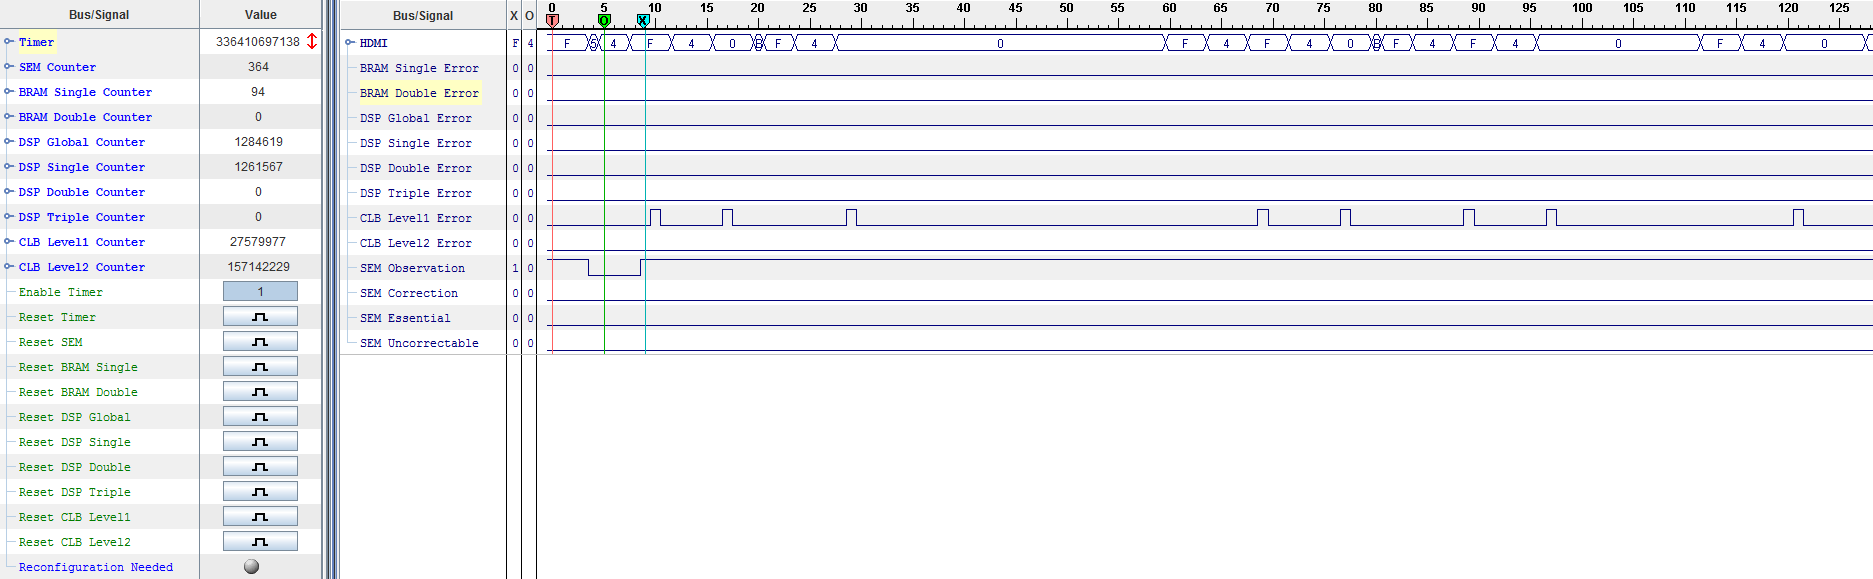
\includegraphics[width=\textwidth]{img/II-6-irradiation/cs-clb.png}
        \caption{.}
        \label{fig:II-6-cs-clb}
      \end{sidewaysfigure}

      The VIO window provides an overview of the error counters and allows to reset them individually. It also controls a timer which is used to count the elapsed time and a "reconfiguration needed" signal which indicates that the irradiated FPGA requires a hard reset. The ILA monitor displays the incoming bits and the resulting information. The first bus labeled "HDMI" holds the four bits used to encode the error types which can be seen to transition from 0x0 to 0xF and 0x4. The 0xF signals the beginning of a transmission and the 0x4 indicates a CLB level-1 error which in turn raises one of the error flags. The last four buses are connected to the signals of the SEM core.

  \section{Irradiation Setup}

    The irradiation tests were performed at the CYCLONE110 cyclotron at the Université Catholique de Louvain \cite{CYCLOTRON} using a proton beam with energies between 14.4 MeV and 62 MeV. The machine can deliver fluxes up to 2 $ \times $ 10$^8$ particles cm$^{-2}$ s$^{-1}$ with a homogeneity of 10\% within an 80 mm $ \times $ 80 mm beam spot. Figure \ref{fig:II-6-cyclotron} is a photograph of the beam line delivering the protons in the irradiation area in front of which degraders can be placed in order to change the energy of the particles. \\

    \begin{figure}[h!]
      \centering
      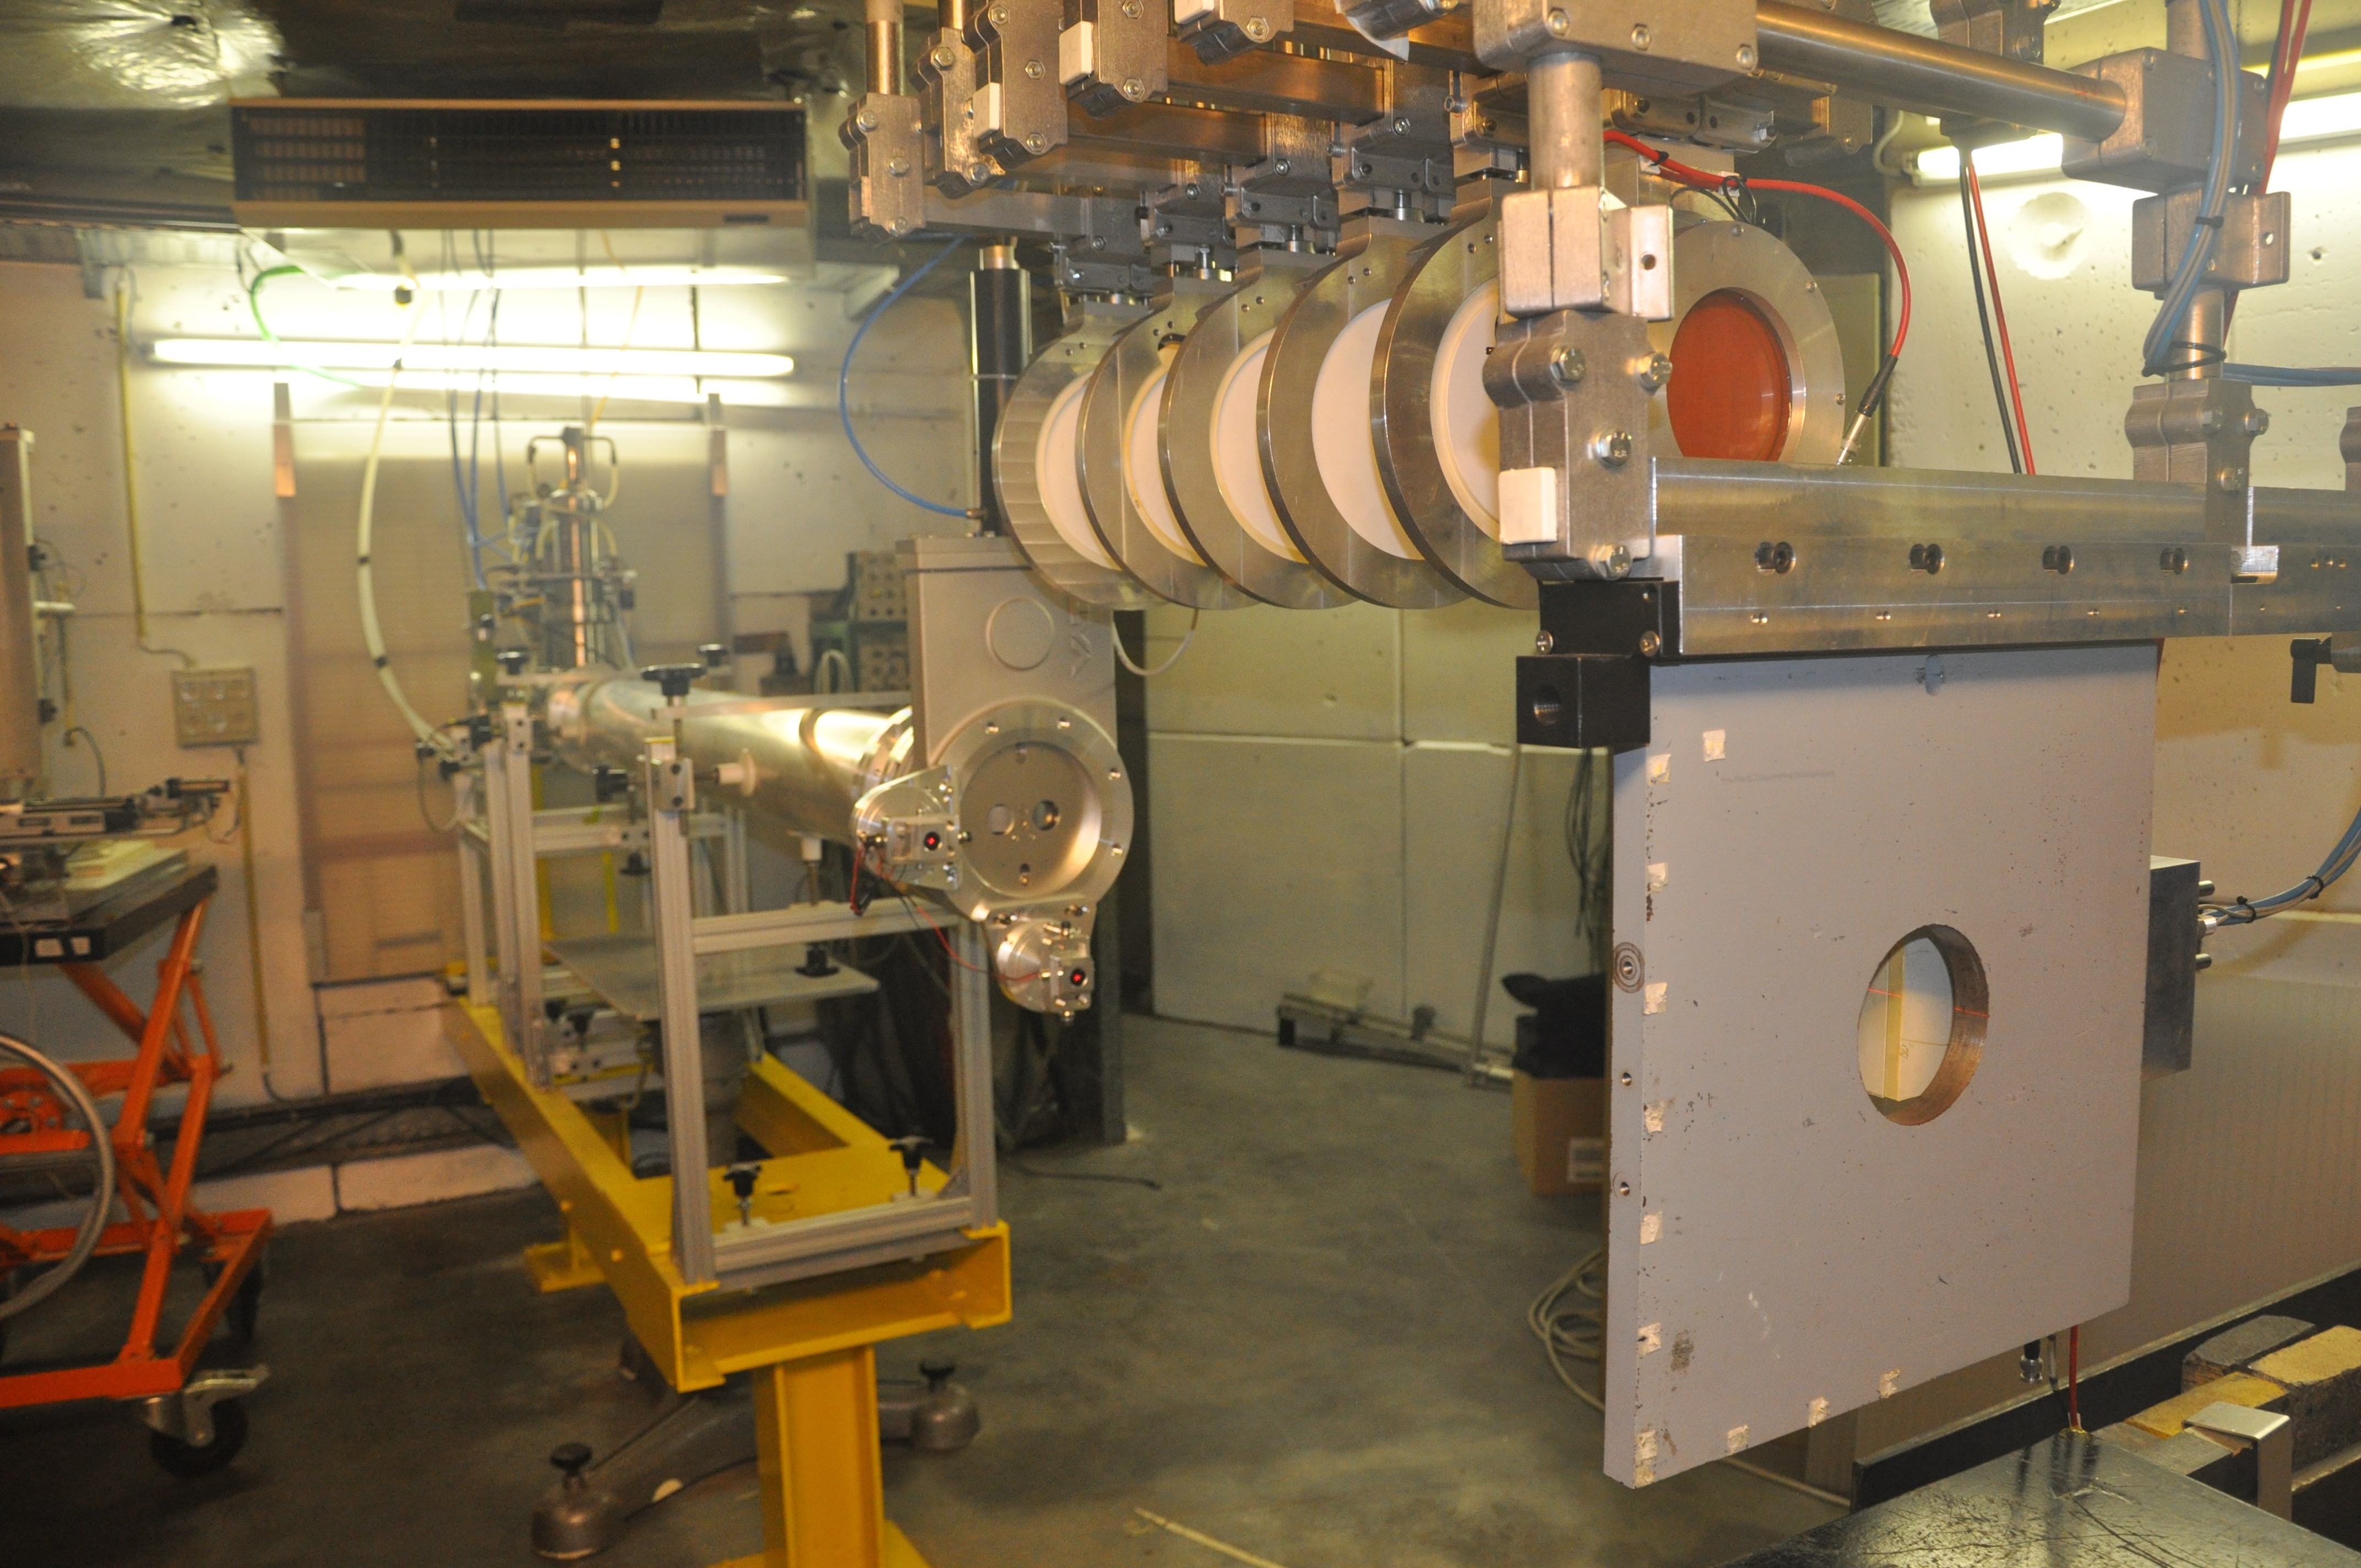
\includegraphics[width=\textwidth]{img/II-6-irradiation/cyclotron.jpg}
      \caption{.}
      \label{fig:II-6-cyclotron}
    \end{figure}

    Two OptoHybrids v2a were installed in front of the beam to mimic the setup of a superchamber in CMS. Figure \ref{fig:II-6-setup} is a photograph of the two boards placed being aligned in front of the beam using lasers. Next to the low voltage cables required the power the board, two HDMI cables are attached to each OptoHybrid v2a: one used to communicate with the control boards, and one used to send reset signals to the FPGA. \\

    \begin{figure}[h!]
      \centering
      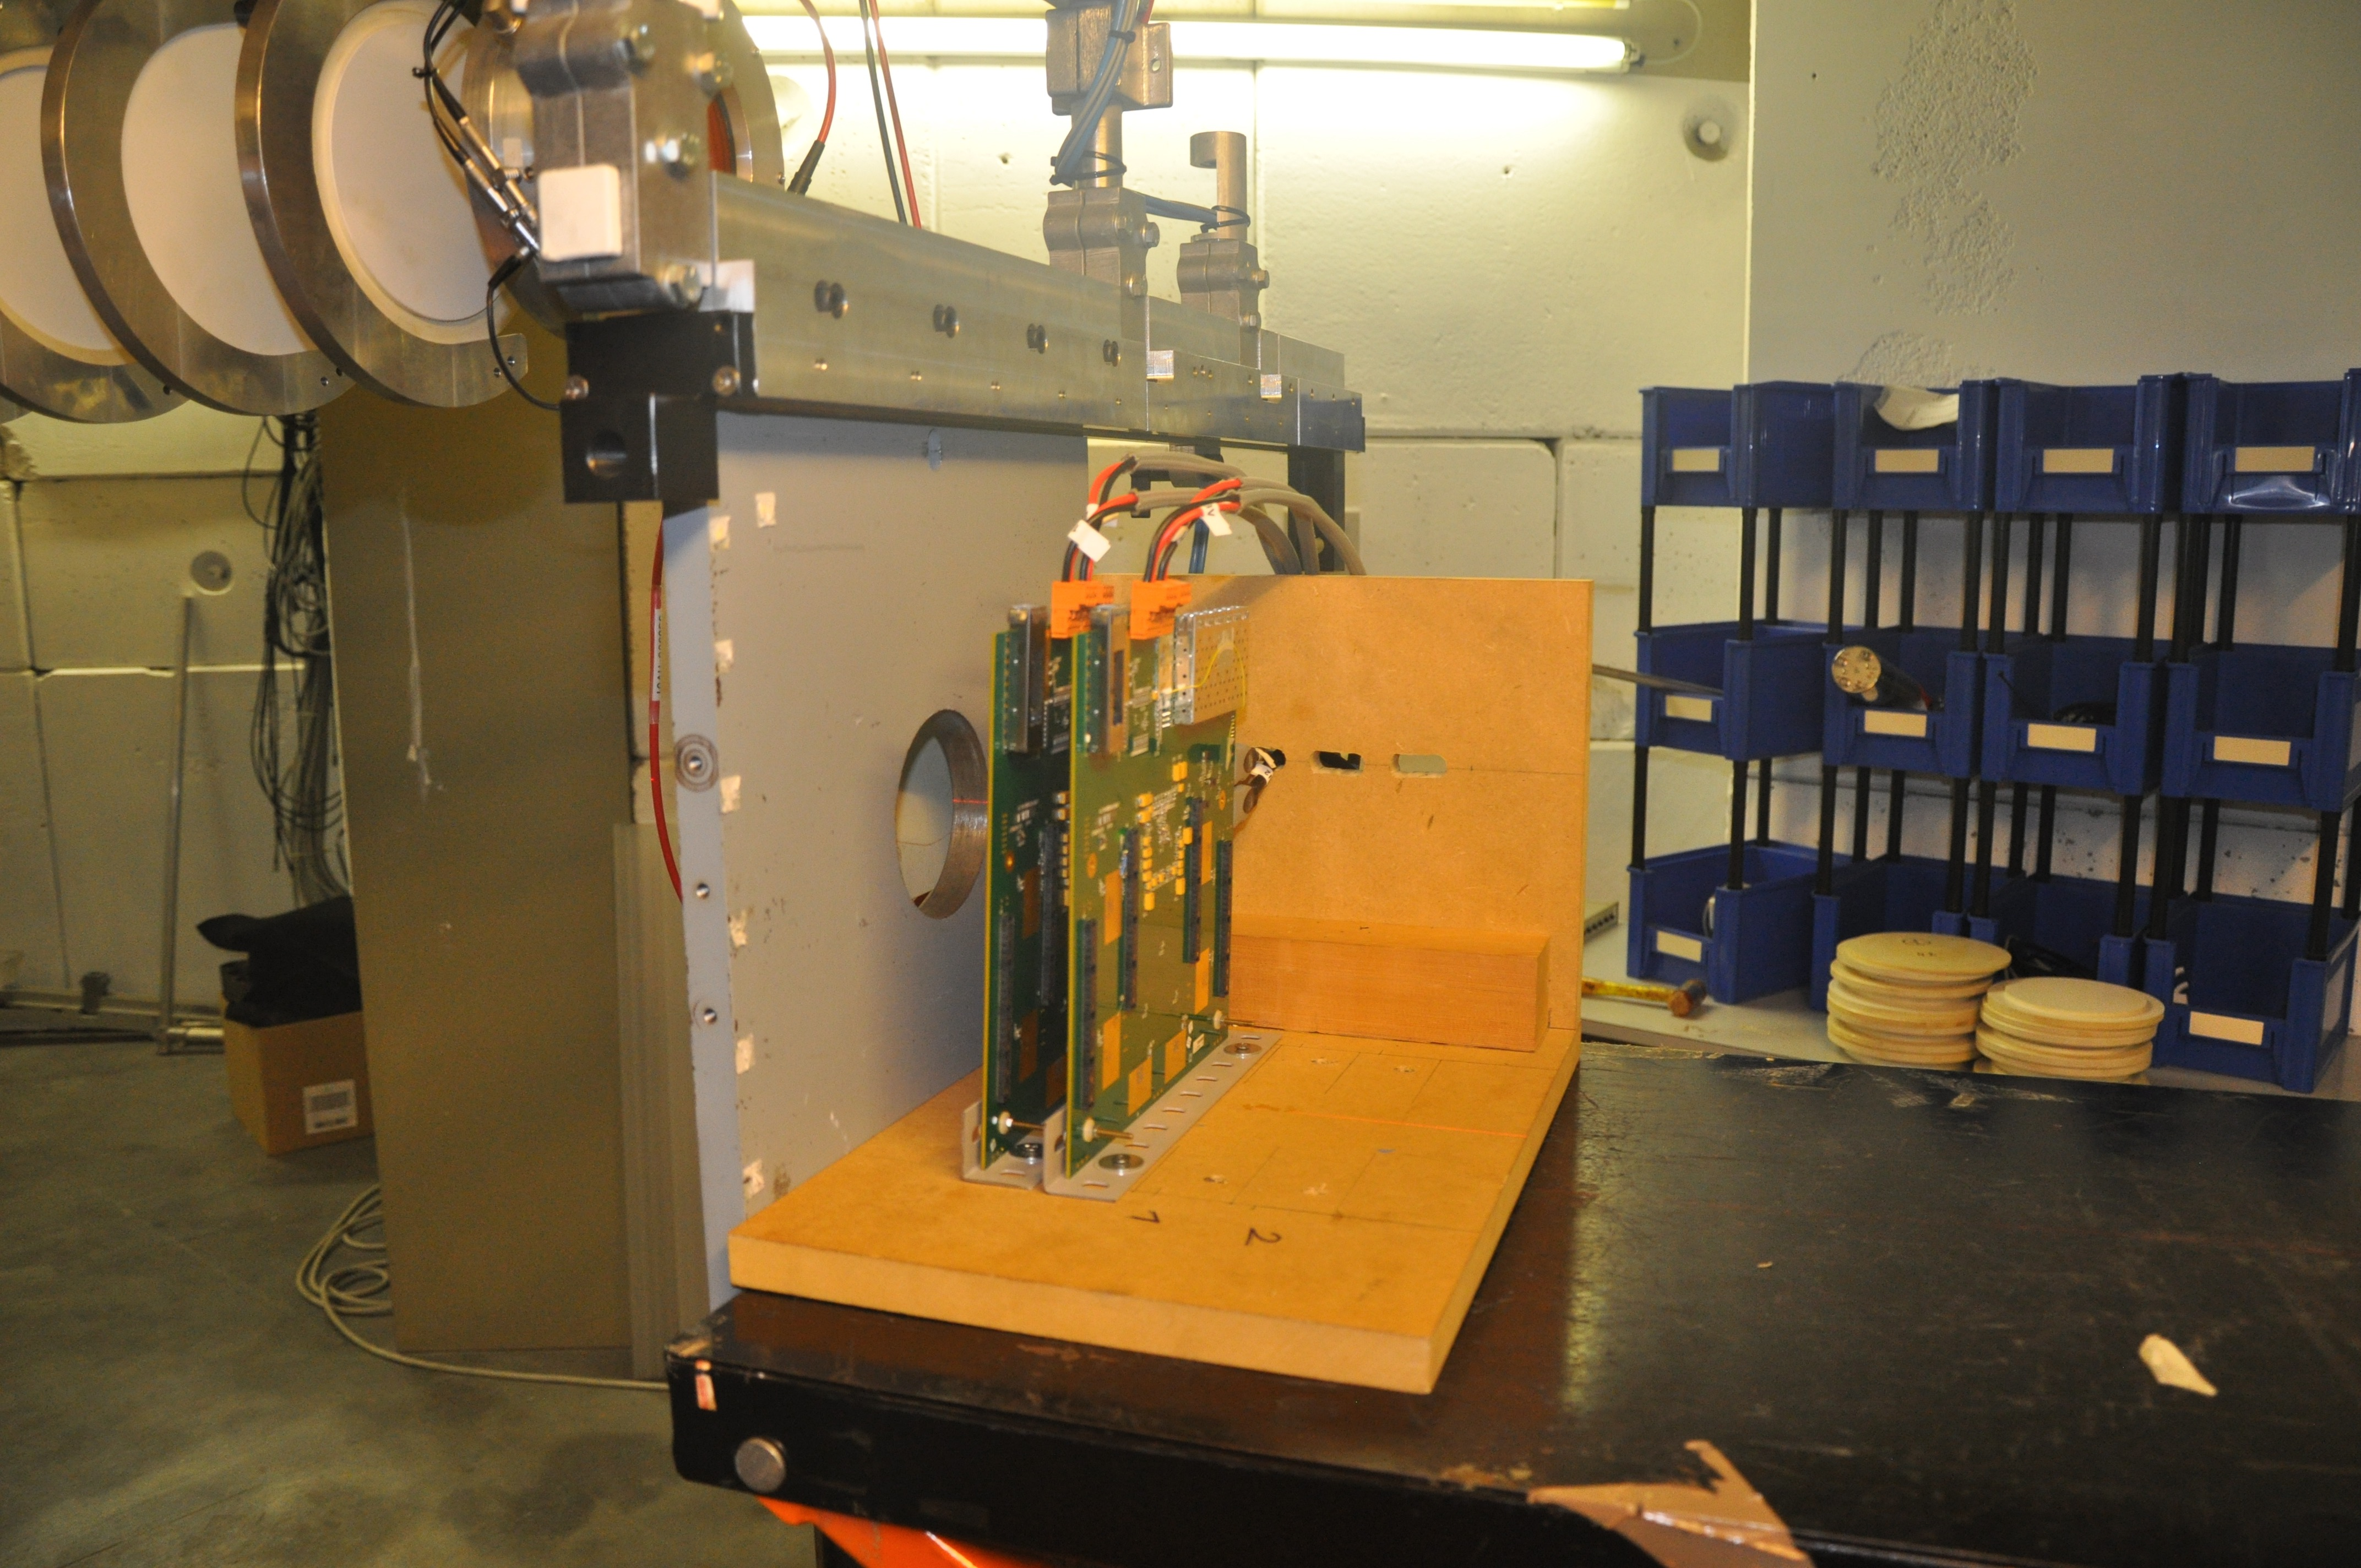
\includegraphics[width=\textwidth]{img/II-6-irradiation/boards.jpg}
      \caption{.}
      \label{fig:II-6-setup}
    \end{figure}

    In the control room, two additional OptoHybrids v2a were used to collect data through the HDMI cable. Data acquisition was performed using ChipScope on the two control boards separately.

  \section{Data Analysis}

  \cite{Bylsma2013242}

    \subsection{Evolution of the SEU Cross Section with the Energy}

      \begin{figure}[h!]
        \centering
        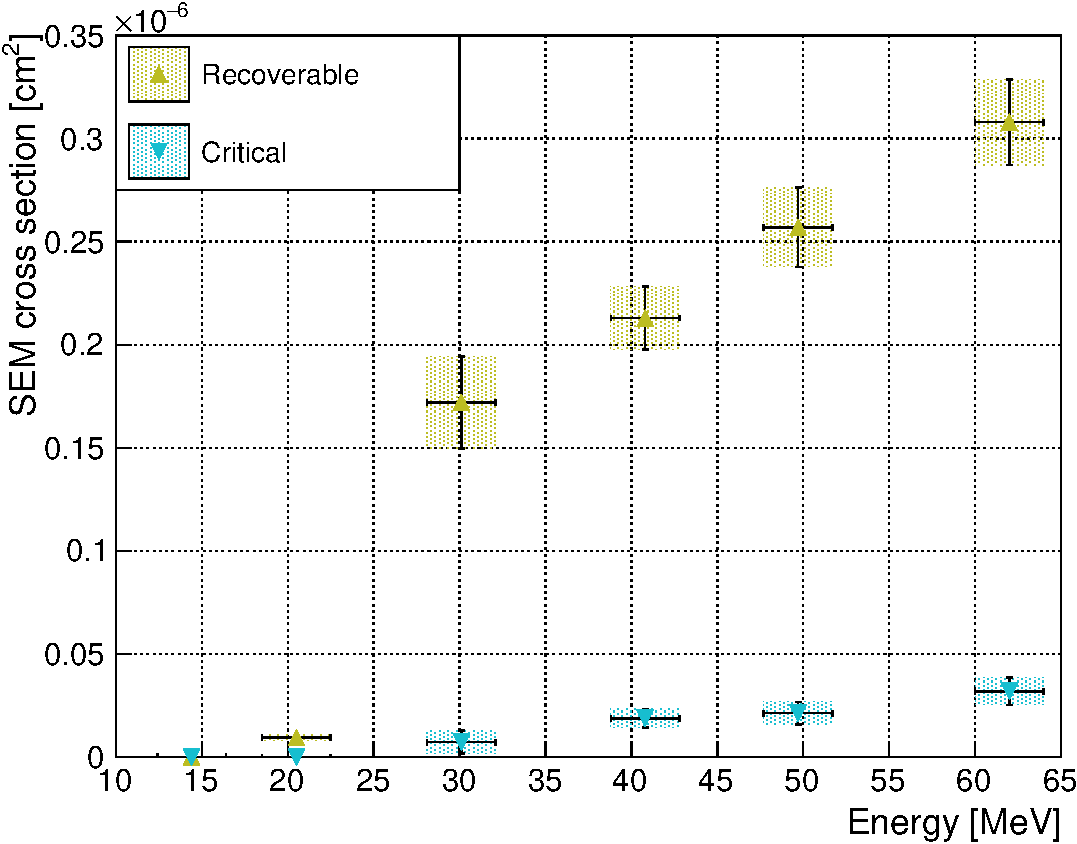
\includegraphics[width=0.49\textwidth]{img/plots/cE_SEM-crop}
        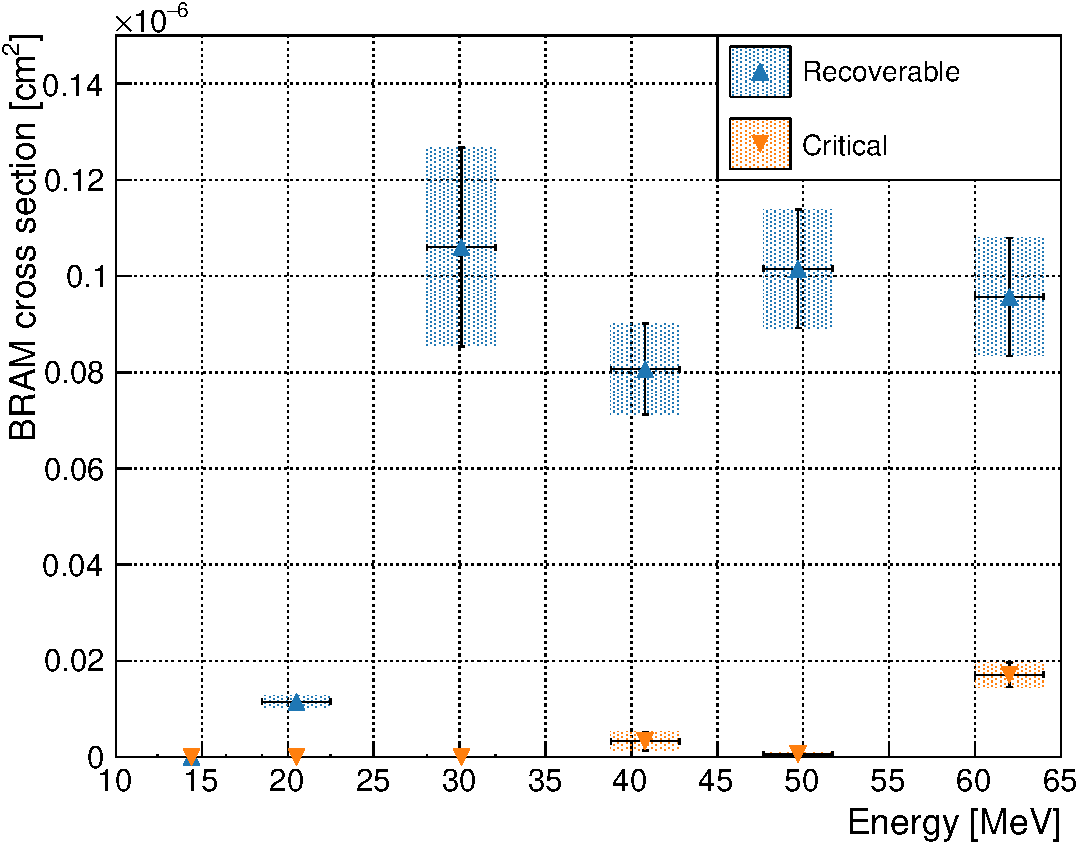
\includegraphics[width=0.49\textwidth]{img/plots/cE_BRAM-crop}
        \caption{Plots of the measured noise (green), measured efficiency (blue), computed efficiency (orange), and tracking data based efficiency (purple) as a function of the VFAT2 threshold in terms of VFAT2 units for GEM0 on the left and GEM1 on the right with muons.}
        \label{fig:II-6-data-seu-energy}
      \end{figure}

    \subsection{Evolution of the SEU Cross Section with the TID}

      \begin{figure}[h!]
        \centering
        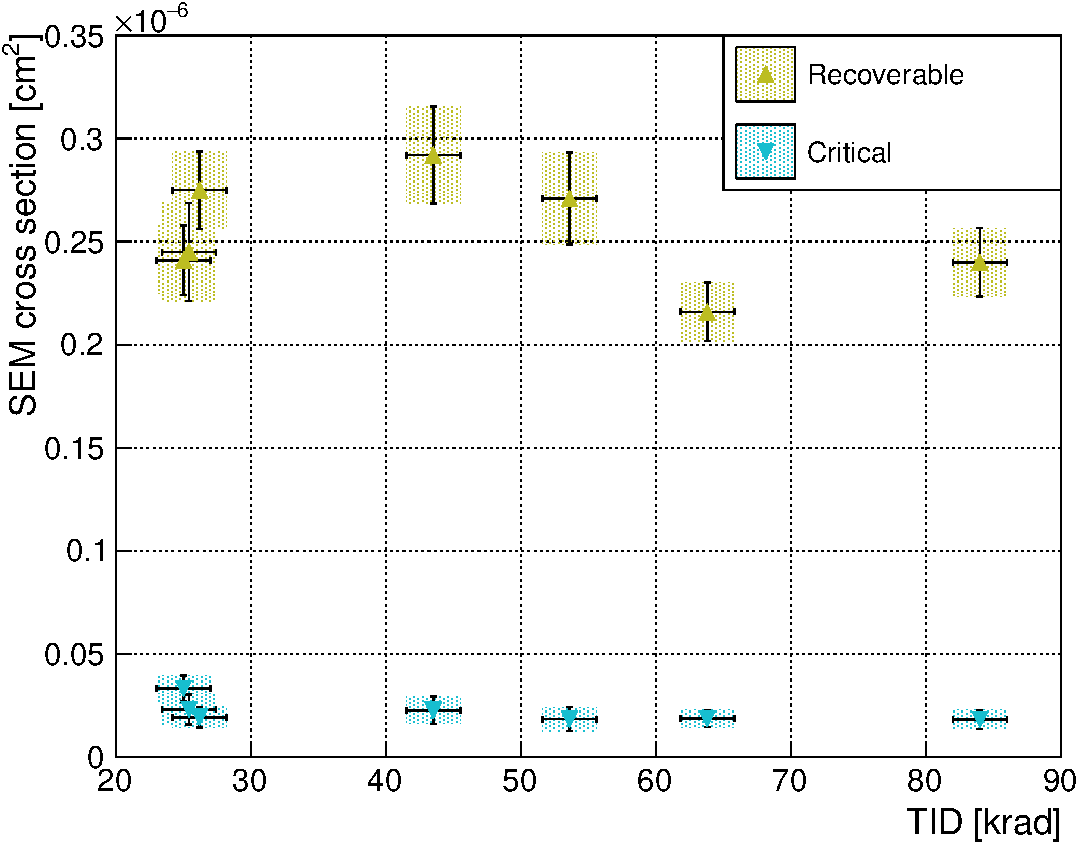
\includegraphics[width=0.49\textwidth]{img/plots/cDose_SEM-crop}
        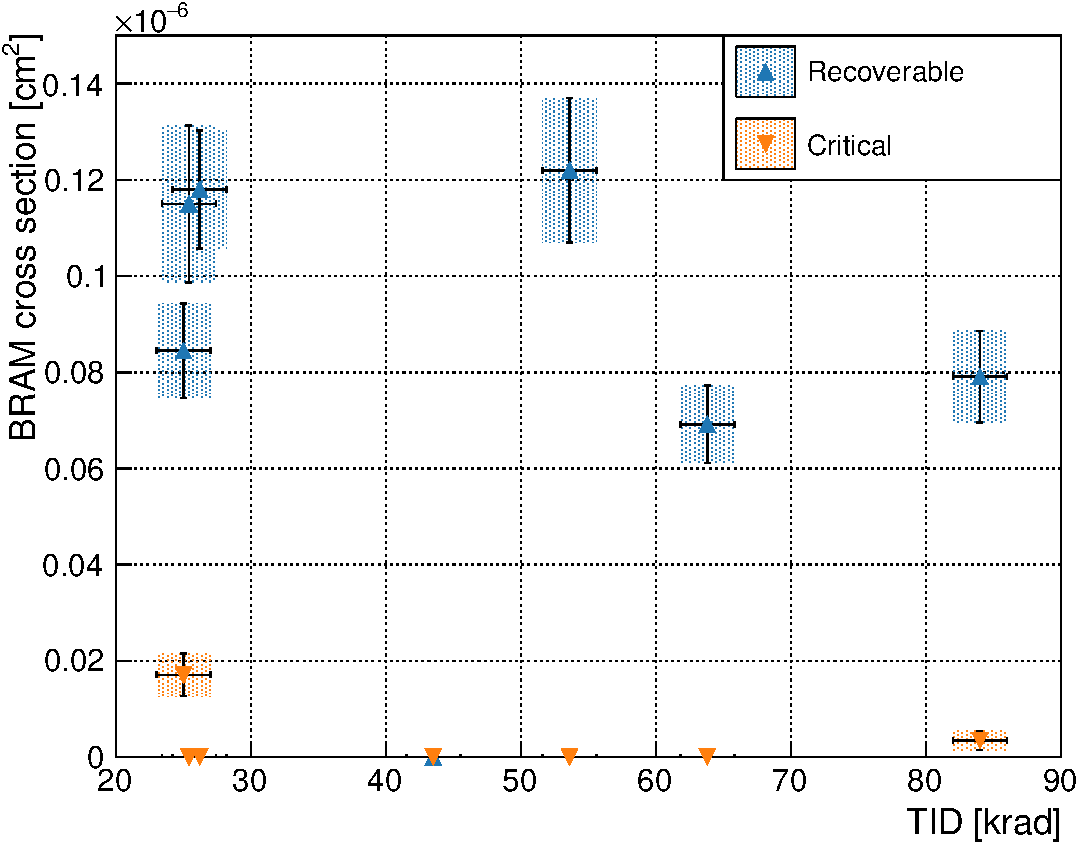
\includegraphics[width=0.49\textwidth]{img/plots/cDose_BRAM-crop}
        \caption{Plots of the measured noise (green), measured efficiency (blue), computed efficiency (orange), and tracking data based efficiency (purple) as a function of the VFAT2 threshold in terms of VFAT2 units for GEM0 on the left and GEM1 on the right with muons.}
        \label{fig:II-6-data-seu-tid}
      \end{figure}

    \subsection{Comparison of the Two Boards}

      \begin{figure}[h!]
        \centering
        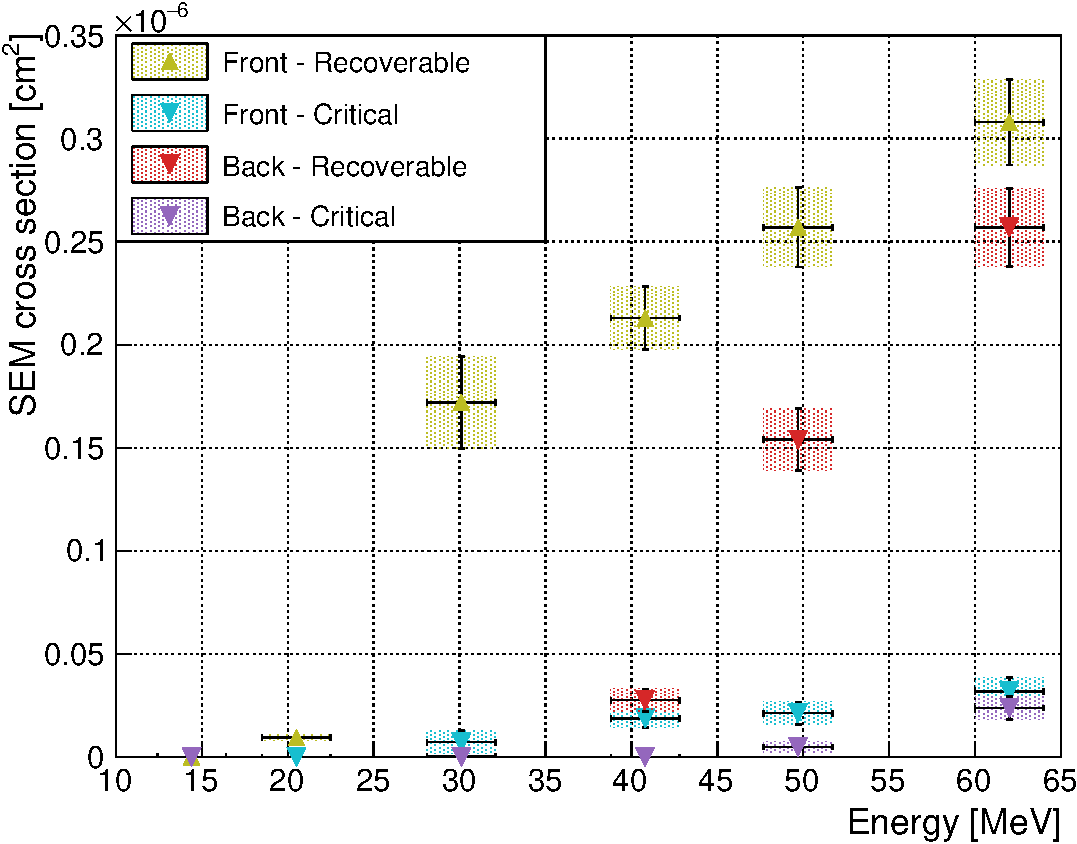
\includegraphics[width=0.49\textwidth]{img/plots/cE_SEU_Comp-crop}
        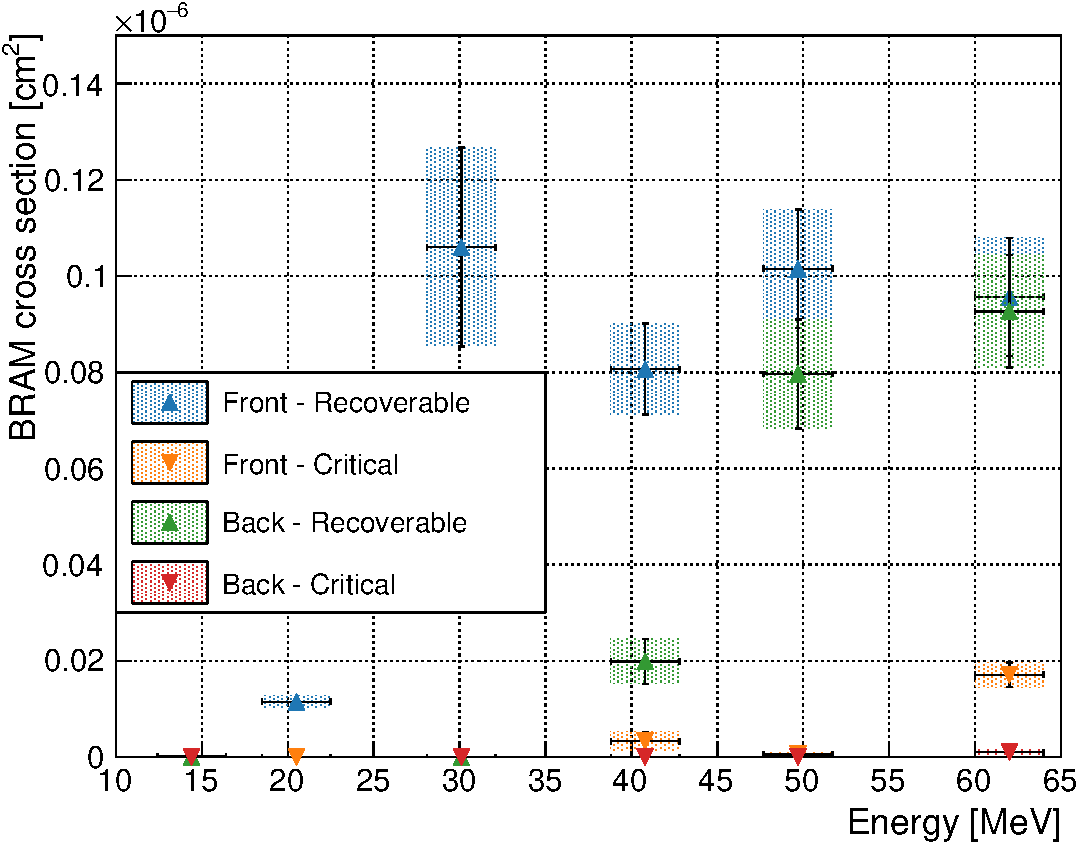
\includegraphics[width=0.49\textwidth]{img/plots/cE_BRAM_Comp-crop}
        \caption{Plots of the measured noise (green), measured efficiency (blue), computed efficiency (orange), and tracking data based efficiency (purple) as a function of the VFAT2 threshold in terms of VFAT2 units for GEM0 on the left and GEM1 on the right with muons.}
        \label{fig:II-6-data-seu-comp}
      \end{figure}

  \section{Conclusion}
